\RequirePackage{luatex85}
\documentclass[paper=a4,fontsize=10.5pt]{jlreq}
\usepackage{amsmath,amsfonts,amssymb,mathtools,ascmac,bm,fancybox,calc,multicol,physics,array}
\usepackage[top=20truemm,bottom=20truemm,left=15truemm,right=15truemm]{geometry}
\usepackage{graphicx,color}
\usepackage{tikz,listings,wrapfig,float,xcolor}
\usepackage{url,subcaption,multirow,framed,comment}
\usepackage[unicode,hidelinks,pdfusetitle]{hyperref}
\usepackage{luatexja-fontspec,lltjext}
\usepackage{TeachersGuide}
\hypersetup{
    colorlinks=true,
    citecolor=black,
    linkcolor=black,
    urlcolor=blue
}
\lstset{
        %プログラム言語(複数の言語に対応,C,C++も可)
    language =TeX,
        %背景色と透過度
    %backgroundcolor={\color[gray]{.90}},
        %枠外に行った時の自動改行
    breaklines = true,
        %自動改行後のインデント量(デフォルトでは20[pt])
    breakindent = 10pt,
        %標準の書体
    basicstyle = \ttfamily\small,
        %コメントの書体
    commentstyle = {\ttfamily \color[cmyk]{1,0.4,1,0}},
        %関数名等の色の設定
    classoffset = 0,
        %キーワード(int, ifなど)の書体
    keywordstyle = {\bfseries \color[cmyk]{1,1,1,1}},
        %表示する文字の書体
    stringstyle = {\ttfamily \color[rgb]{0,0,1}},
        %枠 tは上に線を記載, Tは上に二重線を記載
        %他オプション:leftline,topline,bottomline,lines,single,shadowbox
    frame = leftline,
        %frameまでの間隔(行番号とプログラムの間)
    framesep = 5pt,
        %行番号の位置
    % numbers = left,
        %行番号の間隔
    stepnumber = 1,
        %行番号の書体
    numberstyle = \small,
        %タブの大きさ
    tabsize = 4,
        %キャプションの場所(tbならば上下両方に記載)
    captionpos = t
}
    \usetikzlibrary{intersections,calc,arrows.meta,backgrounds,shapes.geometric,shapes.misc,positioning,fit,graphs,arrows}
    \setlength{\columnsep}{5mm}

    \columnseprule=0.1mm
    \ltjsetparameter{jacharrange={-2}} %日本語以外を欧文扱い

    \renewcommand{\thefootnote}{*\arabic{footnote}}
    \renewcommand{\figurename}{Fig\ }
    \renewcommand{\tablename}{Tbl}
    \newcommand{\figref}[1]{Fig\ \ref{#1}}
    \newcommand{\tabref}[1]{Tbl\ \ref{#1}}

\makeatletter
    \renewcommand{\thefigure}{%
    \thesection.\arabic{figure}}
    \@addtoreset{figure}{section}

    \renewcommand{\thetable}{%
    \thesection.\arabic{table}}
    \@addtoreset{table}{section}

    \@addtoreset{lstlisting}{section}
\makeatother


\title{\vspace{-2em}\textbf{学習指導案}\\ \LaTeXe スタイルファイル 仕様書}
\author{MIZOGUCHI Koki\thanks{Kochi University of Technology}}
\date{\today}


\begin{document}
\maketitle
\begin{leftbar}
    \section*{ファイル情報}
\end{leftbar}
\begin{multicols}{2}
    \noindent\textbf{スタイルファイル名}\\
    \hspace{0.5em}\verb|TeachersGuide.sty|\\
    \textbf{制作者}\\
    \hspace{0.5em}溝口洸熙\\
    \textbf{LICENSE}\\
    \hspace{0.5em}\verb|MIT License|\\
    \newline
    \textbf{更新}
    \begin{itemize}
        \item {\scriptsize\href{https://github.com/MIZOGUCHIKoki/LaTeX-StyleFile}{https://github.com/MIZOGUCHIKoki/LaTeX-StyleFile}}\\
        \item 2020年10月10日以前の\LaTeX では使用不可.\\
        \item (u)p\LaTeX \footnotemark, X\hspace{-0.15em}\raisebox{-0.5ex}[1ex][0ex]{\reflectbox{E}}\hspace{-0.15em}\TeX, Lua\LaTeX 対応.
    \end{itemize}
\end{multicols}
\footnotetext{dvipdfmxオプションが必要}
\begin{leftbar}
    \section*{コマンド・環境定義}
\end{leftbar}
\noindent\ovalbox{\verb|\guideTitle|} [引数:0]\par
タイトル「学習指導案」を出力.変更は\verb| \renewcommand{\guideTitle}{任意のタイトル名} |で可能.\\
\ovalbox{\verb|\showTitle|} [引数:5]\par
タイトルと授業情報を出力.引数には,日付・学級・指導科目・使用教科書・授業者 を入力.\\
\noindent\ovalbox{\verb|\unitTitle|} [引数:1]\par
単元名を出力する.出力方法は,\verb|\unitTitle{単元名}|.\\
\noindent\ovalbox{\verb|UnitGoals|環境}\par
単元の目標を出力.環境内に記述したものを,題名とともに出力.この環境は\verb|quote|環境内にある.\\
\ovalbox{\verb|UnitView|環境}\par
単元観を出力.環境内に記述したものを,題名とともに出力.この環境は\verb|quote|環境内にある.\\
\ovalbox{\verb|EvaluationCriterion|環境}\par
評価規準を出力.この環境は\verb|longtable|内にある.従って,\verb|tabular|環境同様,列の操作は\verb| & |,行の操作は\verb| \\ |で行う.\par
また,各評価の数字付き箇条書きを容易にするため,以下の3つのコマンドを定義した.
\begin{quote}
    \noindent\ovalbox{\verb|\enumiA|},\ovalbox{\verb|\enumiB|},\ovalbox{\verb|\enumiC|}\par
    \ \ これらのコマンドは,数字付き箇条書きの数字の前にそれぞれのアルファベット\verb|A, B, C|を付するコマンドである.\verb|enumirate|環境内で利用する.
\end{quote}
\ \ 評価基準は,左の列から「知識・技能」「思考・判断・表現」「主体的に学習に取り組む態度」である.\\
\ovalbox{\verb|UnitPlan|環境}\par
単元計画を出力.この環境は\verb|longtable|内にある.従って,\verb|tabular|環境同様,列の操作は\verb| & |,行の操作は\verb| \\ |で行う.\par
時間表示を容易にするため,\ovalbox{\verb|\timeCount|}を作成した.呼び出し都度インクリメントするカウンタが\(n\)である時,\verb|"第|\(n\)\verb|時間"|と出力する.\par
単元計画は,左の列から,「時間」「学習活動」「評価規準」「評価方法」である.\\
\ovalbox{\verb|StudentFacts|環境}\par
生徒の実態を出力する.環境内に記述したものを,題名とともに出力.この環境は\verb|quote|環境内にある.\\
\ovalbox{\verb|ClassGoal|環境}\par
本時の到達目標を出力する.環境内に記述したものを,題名とともに出力.この環境は\verb|quote|環境内にある.\\
\ovalbox{\verb|ClassPoint|環境}\par
本時のポイントを出力する.環境内に記述したものを,題名とともに出力.この環境は\verb|quote|環境内にある.\\
\noindent\ovalbox{\verb|TeachingProcedures|環境}\par
指導案表の枠を設計する.この環境は\verb|longtable|環境を用いて構築している.従って\verb|tabular|環境同様,列の区切りは\verb| & |を用い,行の区切りは,\verb|\\ |で行う.\par
ヘッダの部分\footnote{デフォルトでは,活動・指導内容・指導上の留意点及び評価}は,それぞれ括弧内のコマンド\footnote{tpf,tps,tpt}で定義しているので,変更したい場合は,適宜\verb| \renewcommand |\footnote{「活動」を「活動内容」に変更したい場合は,{\ttfamily\textbackslash renewcommand\{\textbackslash tpf\}\{活動内容\}}}で更新する.\vspace{0.5em}\\
\ovalbox{\verb|tpfcol,tpscol,tptcol|環境}\par
\verb|tpf, tps, tpt|の列に対して,\verb|tpfcol,tpscol,tptcol|の環境下で編集を行う.これらは,\verb|minipage|環境を用いて構築している.\par
\newpage
\begin{leftbar}
    \section*{作成例}
\end{leftbar}
\noindent{\small\url{http://www.tochigi-edu.ed.jp/icnt/kenshu-c-h29/?action=common_download_main&upload_id=12782}参考}\\
\hrulefill\vspace{1em}
\showTitle{9月1日 1校時}{3年A組}{数学I}{数学I 数研出版}{溝口洸熙}
\unitTitle{二次関数「二次関数とそのグラフ」}
\begin{UnitGoals}
    \begin{itemize}
        \item 表,式,グラフなどを用いて数量の変化を表現することの有用性を認識し,関数の考えを具体的な事象の考察に活用しようとする.
        \item 関数の概念\dots
    \end{itemize}
\end{UnitGoals}
\begin{UnitView}
    \ \ 二次関数は,高校数学の中で最も基礎的であり,かつ重要な単元である.二次関数を扱い,関数概念の理解を深め,関数を用いて数量の変化を表現することの有用性を認識できるよう\dots
\end{UnitView}
\begin{EvaluationCriterion}
    \begin{enumerate}
        \enumiA
        \item 知識があるといいね
        \item 技能があるといいね
    \end{enumerate} &
    \begin{enumerate}
        \enumiB
        \item 思考があるといいね
        \item 判断があるといいね
        \item 表現があるといいね
    \end{enumerate} &
    \begin{enumerate}
        \enumiC
        \item 主体的に学習に取り組む態度があるといいね
    \end{enumerate}\\
    \hline
\end{EvaluationCriterion}
\begin{UnitPlan}
    \timeCount & 関数の定義について学び,関数の値,値域を求める.& \fbox{A1},\fbox{B2} & 観察・小テスト・自己評価\\
    \hline
    \timeCount & 関数のグラフの意味について学び,1時間数の最大値と最小値を求める.& \fbox{B1},\fbox{B2} & 観察・ワークシート\\
    \hline
    \timeCount & 二次関数\(y=ax^2,y=ax^2+q\)のグラフを描く. & \fbox{A2},\fbox{B1} & 観察・ワークシート・自己評価\\
\end{UnitPlan}
\begin{StudentFacts}
    \ \ 中学校で習った一次関数\(y=ax+b\)や二次関数\(y=ax^2\)に対して苦手意識のある生徒が多く,グラフをかくことができない,関数とグラフの関係が分からないという生徒もいる.\par
    \ \ また,\dots
\end{StudentFacts}
\begin{ClassGoal}
    \begin{itemize}
        \item \(x\)軸方向へ平行移動する二次関数のグラフについて関心をもち,調べようとする.\fbox{C1}
        \item 二次関数 \(y=ax2\)を\(x\)軸方向へ\(p\)だけ平行移動したグラフから二次関数の式を考察できる.\fbox{B1}
    \end{itemize}
\end{ClassGoal}
\begin{ClassPoint}
    \ \ 二次関数$y=a(x-p)^2$のグラフを考えるに当たって,先に式を与えてグラフをかかせることが一般的であるが,\dots
\end{ClassPoint}
\begin{TeachingProcedures}
    \begin{tpfcol}
        \textbf{導入}\\
        前時学習内容の確認
    \end{tpfcol} &
    \begin{tpscol}
        \begin{framed}
            \noindent\underline{復習}\\
            \(y=2x^2-2\)のグラフをかき,頂点と座標の軸の方程式を求めよ.
        \end{framed}
    \end{tpscol} &
    \begin{tptcol}
        \begin{itemize}
            \item 前時の評価を基に,\dots
        \end{itemize}
    \end{tptcol}\\
    \hline
    \begin{tpfcol}
        \textbf{展開}\\
        グラフから関数\[y=a(x-p)^2\]を推測する.
    \end{tpfcol} &
    \begin{tpscol}
        \begin{framed}
            \noindent\underline{課題1}\\
            二次関数\(y-2x^2\)のグラフを\(x\)軸方向に1だけ平行移動したグラフを描く.
        \end{framed}
        \begin{center}
            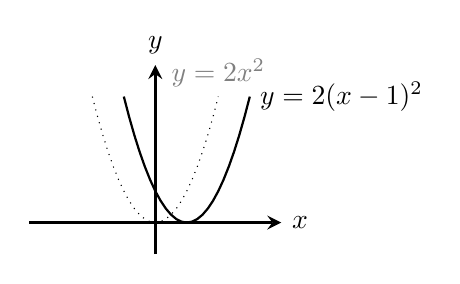
\begin{tikzpicture}[scale=0.4]%倍率
                \draw[very thick, -stealth] (-4,0)--(4,0) node[right] {$x$};%x軸
                \draw[very thick, -stealth] (0,-1)--(0,5) node[above] {$y$};%y軸
                \draw[domain=-2:2,dotted] plot(\x, {pow(\x,2)})node[above]{\textcolor{gray}{\(y=2x^2\)}};
                \draw[domain=-1:3,thick] plot(\x, {pow(\x,2)-2*\x+1})node[right]{{\(y=2(x-1)^2\)}};
            \end{tikzpicture}
        \end{center}
        \vspace{0.5em}
        \begin{equation}
            \begin{aligned}
                2(x-1)^2 & = 2(x^2-2x+1) \\
                         & = 2x^2-4x+2
            \end{aligned}
        \end{equation}
    \end{tpscol} &
    \begin{tptcol}
        \begin{framed}
            \noindent\textbf{評価}\\ {\small(主体的に学習に取り組む態度)}\\
            \(x\)軸方向へ平行移動する二次関数のグラフについて関心を持ち,調べようとする.
            \rightline{\fbox{C1}}
        \end{framed}
    \end{tptcol}\vspace{3em}\\
    &&\\
    \hline
    \begin{tpfcol}
        \textbf{振り返り}\\
        二次関数の式とグラフの平行移動について理解する.
    \end{tpfcol} &
    \begin{tpscol}
        \begin{framed}
            \noindent\underline{発展問題}\\
            二次関数\(y=2(x-p)^2\)のグラフは,\(y=2x^2\)のグラフをどのように平行移動したグラフとなるか.
        \end{framed}
    \end{tpscol} & \\
    \begin{tpfcol}
        自己評価をする.
    \end{tpfcol} &
    \begin{tpscol}
        自己評価表を記入する.
    \end{tpscol} &
    \begin{tptcol}
        自己評価表を活用する.
    \end{tptcol} \\
    \hline
\end{TeachingProcedures}
\newpage
\begin{center}
    \LaTeX ソースコード
\end{center}
\begin{lstlisting}
\documentclass{jlreq}
\usepackage{TeachersGuide}
%%%%
% 他プリアンブルは略
%%%%
\begin{document}
\showTitle{9月1日 1校時}{3年A組}{数学I}{数学I 数研出版}{溝口洸熙}
\unitTitle{二次関数「二次関数とそのグラフ」}
\begin{UnitGoals}
    \begin{itemize}
        \item 表,式,グラフなどを用いて数量の変化を表現することの有用性を認識し,関数の考えを具体的な事象の考察に活用しようとする.
        \item 関数の概念\dots
    \end{itemize}
\end{UnitGoals}
\begin{UnitView}
    \ \ 二次関数は,高校数学の中で最も基礎的であり,かつ重要な単元である.二次関数を扱い,関数概念の理解を深め,関数を用いて数量の変化を表現することの有用性を認識できるよう\dots
\end{UnitView}
\begin{EvaluationCriterion}
    \begin{enumerate}
        \enumiA
        \item 知識があるといいね
        \item 技能があるといいね
    \end{enumerate} &
    \begin{enumerate}
        \enumiB
        \item 思考があるといいね
        \item 判断があるといいね
        \item 表現があるといいね
    \end{enumerate} &
    \begin{enumerate}
        \enumiC
        \item 主体的に学習に取り組む態度があるといいね
    \end{enumerate}\\
    \hline
\end{EvaluationCriterion}
\begin{UnitPlan}
    \timeCount & 関数の定義について学び,関数の値,値域を求める.& \fbox{A1},\fbox{B2} & 観察・小テスト・自己評価\\
    \hline
    \timeCount & 関数のグラフの意味について学び,1時間数の最大値と最小値を求める.& \fbox{B1},\fbox{B2} & 観察・ワークシート\\
    \hline
    \timeCount & 二次関数\(y=ax^2,y=ax^2+q\)のグラフを描く. & \fbox{A2},\fbox{B1} & 観察・ワークシート・自己評価\\
\end{UnitPlan}
\begin{StudentFacts}
    \ \ 中学校で習った一次関数\(y=ax+b\)や二次関数\(y=ax^2\)に対して苦手意識のある生徒が多く,グラフをかくことができない,関数とグラフの関係が分からないという生徒もいる.\par
    \ \ また,\dots
\end{StudentFacts}
\begin{ClassGoal}
    \begin{itemize}
        \item \(x\)軸方向へ平行移動する二次関数のグラフについて関心をもち,調べようとする.\fbox{C1}
        \item 二次関数 \(y=ax2\)を\(x\)軸方向へ\(p\)だけ平行移動したグラフから二次関数の式を考察できる.\fbox{B1}
    \end{itemize}
\end{ClassGoal}
\begin{ClassPoint}
    \ \ 二次関数$y=a(x-p)^2$のグラフを考えるに当たって,先に式を与えてグラフをかかせることが一般的であるが,\dots
\end{ClassPoint}
\begin{TeachingProcedures}
    \begin{tpfcol}
        \textbf{導入}\\
        前時学習内容の確認
    \end{tpfcol} &
    \begin{tpscol}
        \begin{framed}
            \noindent\underline{復習}\\
            \(y=2x^2-2\)のグラフをかき,頂点と座標の軸の方程式を求めよ.
        \end{framed}
    \end{tpscol} &
    \begin{tptcol}
        \begin{itemize}
            \item 前時の評価を基に,\dots
        \end{itemize}
    \end{tptcol}\\
    \hline
    \begin{tpfcol}
        \textbf{展開}\\
        グラフから関数\[y=a(x-p)^2\]を推測する.
    \end{tpfcol} &
    \begin{tpscol}
        \begin{framed}
            \noindent\underline{課題1}\\
            二次関数\(y-2x^2\)のグラフを\(x\)軸方向に1だけ平行移動したグラフを描く.
        \end{framed}
        \begin{center}
            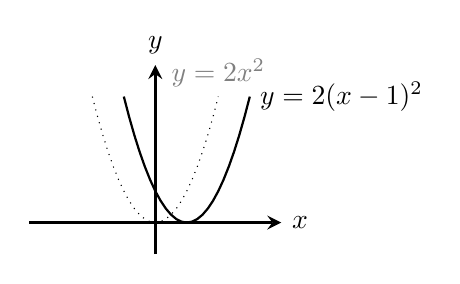
\begin{tikzpicture}[scale=0.4]%倍率
                \draw[very thick, -stealth] (-4,0)--(4,0) node[right] {$x$};%x軸
                \draw[very thick, -stealth] (0,-1)--(0,5) node[above] {$y$};%y軸
                \draw[domain=-2:2,dotted] plot(\x, {pow(\x,2)})node[above]{\textcolor{gray}{\(y=2x^2\)}};
                \draw[domain=-1:3,thick] plot(\x, {pow(\x,2)-2*\x+1})node[right]{{\(y=2(x-1)^2\)}};
            \end{tikzpicture}
        \end{center}
        \vspace{0.5em}
        \begin{equation}
            \begin{aligned}
                2(x-1)^2 & = 2(x^2-2x+1) \\
                         & = 2x^2-4x+2
            \end{aligned}
        \end{equation}
    \end{tpscol} &
    \begin{tptcol}
        \begin{framed}
            \noindent\textbf{評価}\\ {\small(主体的に学習に取り組む態度)}\\
            \(x\)軸方向へ平行移動する二次関数のグラフについて関心を持ち,調べようとする.
            \rightline{\fbox{C1}}
        \end{framed}
    \end{tptcol}\vspace{3em}\\
    &&\\
    \hline
    \begin{tpfcol}
        \textbf{振り返り}\\
        二次関数の式とグラフの平行移動について理解する.
    \end{tpfcol} &
    \begin{tpscol}
        \begin{framed}
            \noindent\underline{発展問題}\\
            二次関数\(y=2(x-p)^2\)のグラフは,\(y=2x^2\)のグラフをどのように平行移動したグラフとなるか.
        \end{framed}
    \end{tpscol} & \\
    \begin{tpfcol}
        自己評価をする.
    \end{tpfcol} &
    \begin{tpscol}
        自己評価表を記入する.
    \end{tpscol} &
    \begin{tptcol}
        自己評価表を活用する.
    \end{tptcol} \\
    \hline
\end{TeachingProcedures}
\end{document}
\end{lstlisting}
\end{document}